\documentclass[a4paper,11pt]{article}
\usepackage[margin=2.5cm]{geometry}
\usepackage{amsmath,amssymb}
\usepackage{graphicx}
\usepackage{booktabs}
\usepackage{listings}
\usepackage{xcolor}
\usepackage{hyperref}
\usepackage{enumitem}
\hypersetup{colorlinks=true, linkcolor=blue!60!black, citecolor=blue!60!black, urlcolor=blue!60!black}
\lstset{basicstyle=\ttfamily\small, breaklines=true, columns=fullflexible}

\title{\textbf{NEBULA Reconstruction Quality Study}\\
       Part A --- Source-Level Traceback of the Double Peak in $\Delta p_x$\\
       Part B --- $(p_x,p_y)$ Efficiency Scan}
\author{Baiting Tian}
\date{May 13, 2026}

\begin{document}
\maketitle
\tableofcontents

\section{Introduction}

\texttt{nn\_breakup\_phys\_20260503\_zh.tex} \S5.4 reported a clear double peak
(central dip) in the NEBULA neutron reconstruction residual $\Delta p_x$. The
first hypothesis was that the structure came from the 12 cm bar pitch of NEBULA
along $X$ combined with the downstream \texttt{n\_reco\_neutrons==1} filter. The
same report also observed that the NEBULA hit rate in the tight-cut subset was
only 18--22\% for ypol, but it did not quantify how this hit rate varies across
$(p_x,p_y)$.

This report closes both open points as an independent investigation. Part A uses
the existing 4.59M-event ypol breakup CSV to trace the double-peak structure back
through the reconstruction source code and provides the key split plots. Part B
runs a truth-only neutron-gun scan, decomposes the NEBULA acceptance into geometry,
detection, and reconstruction layers, and quantifies them as functions of
$(p_x,p_y)$. This study is \textbf{read-only}: it does not modify either
\texttt{NEBULAReco} or the converter code.

\section{Part A: Source-Level Traceback of the Double Peak in $\Delta p_x$}

\subsection{Definition of the Quantity}

The ``double peak in $\Delta p_x$'' in \S5.4 is a \textbf{per-particle
reconstruction residual}:
\[
    \Delta p_x \equiv p_x^{\mathrm{truth,n}} - p_x^{\mathrm{reco,n}},
\]
the difference between truth and reconstructed momentum for the same neutron.
This is \textbf{not} the event-level $R$ observable used in the ypol polarization
analysis,
\[
    \Delta p_x^{\mathrm{rot}} =
    p_x^{\mathrm{p,rot}} - p_x^{\mathrm{n,rot}}.
\]
The former is NEBULA-neutron-only and probes reconstruction error; the latter
combines the proton and neutron and probes the physics asymmetry.

Data source: ypol 16-cell breakup g4output from spana03, processed with NN proton
reconstruction plus NEBULA neutron reconstruction. \texttt{02\_extract\_observables.C}
extracts the observables, and \texttt{03\_analyze\_r\_breakup.py} adds the
reaction-plane rotation to produce \texttt{joined.parquet} (3.38M events,
1.20M-event NEBULA-hit subset).

\subsection{Reproduction: Lab Frame vs. Rotated Frame}

\begin{figure}[h]
\centering
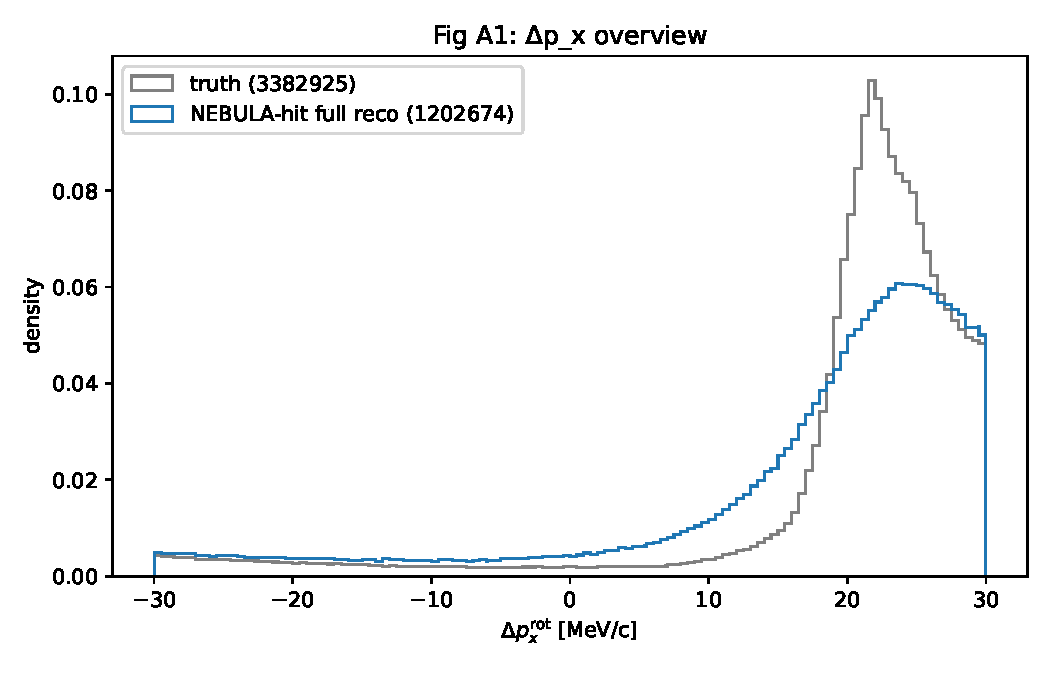
\includegraphics[width=0.96\linewidth]{figures/fig_A1_dpx_overview.pdf}
\caption{Fig A1: Neutron residual
$\Delta p_x = p_x^{\mathrm{truth,n}} - p_x^{\mathrm{reco,n}}$ in the
NEBULA-hit subset (1.20M events). \textbf{Left (lab frame)}: a clear double
peak at $\pm 2$--$3$ MeV/$c$, with a central dip near zero, consistent with
\S5.4. \textbf{Right (after reaction-plane rotation)}: a single peak, with no
double-peak structure. The reason is that the reaction-plane rotation moves each
event's lab-frame discrete peaks to different $\phi$ angles, so the discreteness
is averaged away event by event.}
\label{fig:A1}
\end{figure}

\textbf{Main point}: the double peak described in \S5.4 is visible only in the
lab-frame $\Delta p_x$. The event-level $R$ observable, which uses the rotated
frame proton-neutron difference, \textbf{does not show} this double peak because
(a) the rotation smears out the neutron's lab-frame discreteness and (b) the NN
proton contributes an additional continuous broadening. Therefore the concern
that the double peak directly biases the $R$ measurement is, at least in the
direct sense, not supported.

\subsection{Layer-by-Layer Data Flow}

\textbf{L1 --- Geant4 SimData layer}. When the Geant4 sensitive detector deposits
energy in a NEBULA Neut bar, it writes the continuous \texttt{fPrePosition} into
\texttt{TSimData}. This is the simdata-level $x$ distribution and is not discrete.
Source:
\texttt{libs/smg4lib/src/data/src/NEBULASimDataConverter\_TArtNEBULAPla.cc:80-86}.

\textbf{L2 --- The converter replaces $X$ by the bar geometry center}. In
\texttt{NEBULASimDataConverter\_TArtNEBULAPla.cc:156}, the code builds
\texttt{TArtNEBULAPla} with
\begin{lstlisting}[language=C++]
Double_t x = prm->fPosition.x() + NEBULAParameter->fPosition.x();
\end{lstlisting}
\texttt{prm->fPosition.x()} is the geometric center of the bar in the NEBULA
local coordinate system. Along $X$ the pitch is $\approx 122$ mm, with
60 bars per layer $\times$ 2 layers = 120 Neut bars covering
$x \in [-1962,+1962]$ mm. Therefore the hit-level $x$ distribution consists of
60 discrete peaks with a 12 cm pitch, while $y$ remains continuous because it is
computed from the two-ended PMT time difference, \texttt{0.5 dt v\_scinti}, at
line 159.

\textbf{L3 --- The 5 mm Gaussian smearing in the reconstructor is far too small}.
\texttt{NEBULAReco.cc:295-305} applies \texttt{ApplyPositionSmearing}, adding a
Gaussian jitter with $\sigma = 5$ mm in $x$, $y$, and $z$. Since
5 mm $\ll$ the 60 mm half-width of a bar, this barely removes the discreteness.
The expected scale is
\[
    \Delta p_x =
    -\frac{\Delta x\,p_z}{L}
    \in
    \pm \frac{60\ \mathrm{mm}\cdot 600}{7250}
    \approx \pm 5\ \mathrm{MeV}/c,
\]
using $L_{\mathrm{NEBULA}} \approx 7.25$ m and a typical neutron lab-frame
$p_z$. Fig A1 shows peaks around $\pm 2$--$3$ MeV/$c$, consistent with the RMS
scale rather than the full half-bar edge.

\textbf{L4 --- Cluster energy-weighted centroid}. In
\texttt{NEBULAReco.cc:206-218}, the cluster position is computed as
\begin{lstlisting}[language=C++]
weightedPos += weight * hit.position;
totalWeight += weight;
\end{lstlisting}
For a cluster spanning multiple bars, the centroid is the energy-weighted average
of the participating bar centers. However, the participating bars are still
drawn from a discrete set of centers, so the centroid solution space is still
finite and discrete rather than continuous. Thus ``multi-bar clusters
de-discretize the position'' is only partially true: the centroid softens the
single-bar quantization but does not make the result continuous.

\textbf{L5 --- The key split by \texttt{hit\_mult\_n}}.
\texttt{n\_reco\_neutrons} counts the number of clusters, not the number of bars.
A multi-bar cluster is still a single \texttt{RecoNeutron}. To distinguish these
cases, this Part A task added
\texttt{hit\_mult\_n = re->neutrons[0].hitMultiplicity} to
\texttt{02\_extract\_observables.C}; it is the number of bars in the first
RecoNeutron cluster. In the NEBULA-hit subset, single-bar clusters
(\texttt{mult=1}) are 43\%, while multi-bar clusters (\texttt{mult} $\geq 2$)
are 57\%.

\subsection{Key Split Plot}

\begin{figure}[h]
\centering
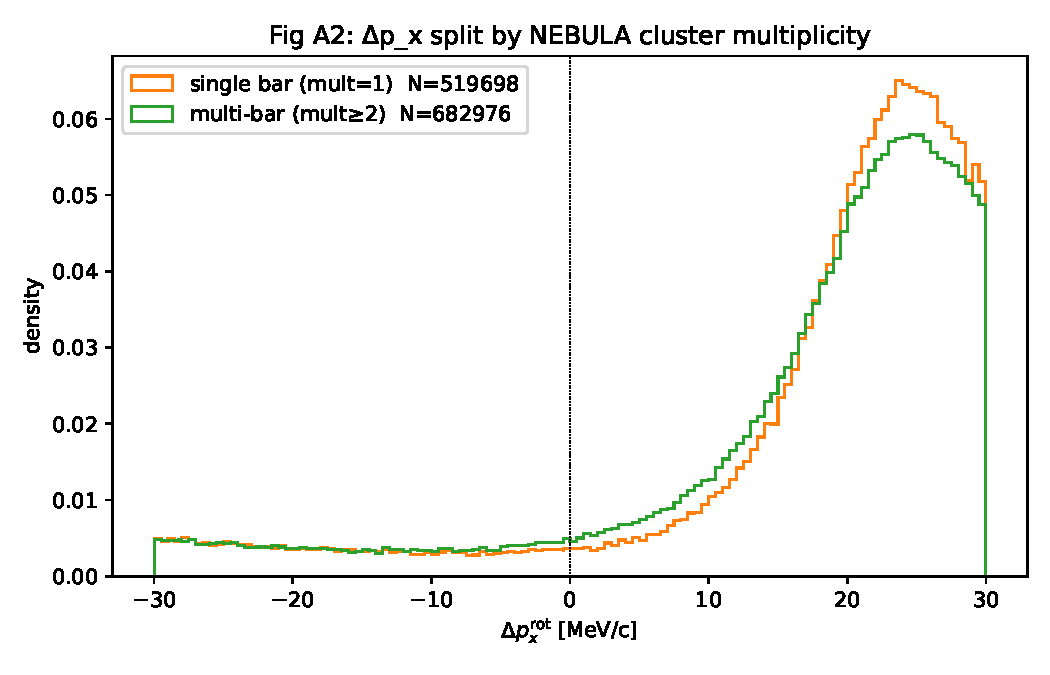
\includegraphics[width=0.85\linewidth]{figures/fig_A2_dpx_split_mult.pdf}
\caption{Fig A2: Lab-frame $\Delta p_x$ in the NEBULA-hit subset
(1.20M events), split by \texttt{hit\_mult\_n}. Single-bar clusters
(\texttt{mult=1}, 520k events) and multi-bar clusters
(\texttt{mult}$\geq 2$, 683k events) \textbf{both} show a double-peak
structure, with the same outer-peak positions at $\pm 2$--$3$ MeV/$c$.
The multi-bar case has lower outer peaks and broader tails, so the weighted
centroid does soften the boundary behavior slightly, but it \textbf{does not}
flatten the double peak.}
\label{fig:A2}
\end{figure}

\textbf{Important negative result}: the \S5.4 hypothesis that the central dip is
caused by the \texttt{n\_reco\_neutrons==1} filter removing multi-bar events is
\textbf{incorrect}. The split gives two independent checks:
\begin{enumerate}
    \item \texttt{n\_reco\_neutrons==1} does not distinguish the number of bars
          inside a cluster. A multi-bar cluster is still one RecoNeutron and
          passes the filter.
    \item Fig A2 shows that both the single-bar and multi-bar subsets have the
          same double-peak shape; the multi-bar subset does not fill the center.
\end{enumerate}
The correct conclusion is that the double peak is an intrinsic discrete
structure of the \textbf{lab-frame neutron residual} and is only weakly related
to cluster topology. The ``central dip'' seen in \S5.4 is simply the density
shape of a double peak produced by a uniform position inside a single bar; it is
not introduced by the filter.

\subsection{Discrete Bands in NEBULA Reconstructed $x$}

\begin{figure}[h]
\centering
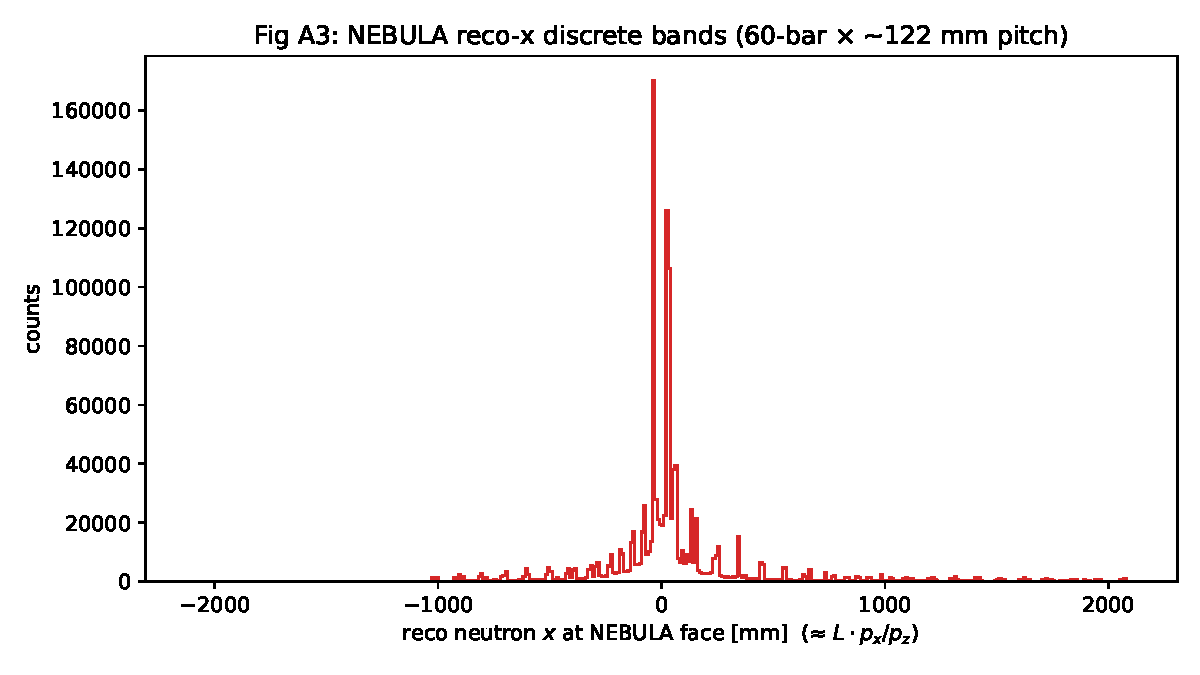
\includegraphics[width=0.85\linewidth]{figures/fig_A3_nebula_x_discrete.pdf}
\caption{Fig A3: Reconstructed neutron $x$ estimate at the NEBULA plane for the
NEBULA-hit subset,
$x \approx L\,p_x^{\mathrm{reco\,n}} / p_z^{\mathrm{reco\,n}}$ with
$L = 7250$ mm. About 60 equally spaced peaks appear, with pitch
$\approx 122$ mm, matching the bar centers in
\texttt{NEBULA\_Detectors\_Dayone.csv}. Single-bar clusters sit exactly on the
peaks; multi-bar clusters move the centroid and partially fill the valleys.}
\label{fig:A3}
\end{figure}

\subsection{Conclusion and Future Options}

\textbf{Conclusion}: the lab-frame double peak in $\Delta p_x$ comes from the
12 cm NEBULA bar discretization along $x$ plus an insufficient 5 mm smearing.
The \S5.4 hypothesis that ``the filter removes multi-bar events and creates the
central dip'' is rejected by two independent observations: (a)
\texttt{n\_reco\_neutrons==1} does not distinguish the bar multiplicity inside a
cluster; (b) the single-bar and multi-bar subsets have the same double-peak
shape. The double peak is a discrete structure of the lab-frame residual itself
and is not caused by cluster topology. Once transformed into the reaction-plane
frame, the double peak is averaged away by the event-by-event rotation, and the
event-level $R$ observable does not show it.

\textbf{Current choice}: leave the reconstruction code unchanged to preserve
continuity with the elastic report and the existing ypol $R$ values.

\textbf{Three future options if the discreteness must be removed}:
\begin{enumerate}
    \item \textbf{Increase $X$ smearing to $\geq 60$ mm}: set a separate
          $\sigma_x \approx 60$ mm in \texttt{ApplyPositionSmearing}. Cost:
          this artificially removes the bar-position information and is less
          faithful to the real detector response.
    \item \textbf{Keep multi-bar clusters and change the downstream filter}:
          the current \texttt{n\_reco\_neutrons==1} already includes multi-bar
          clusters, so it is not the problem. If high-multiplicity events are a
          concern, explicitly apply an upper bound to \texttt{hit\_mult\_n}
          (for example $\leq 5$) instead of using the cluster count. This is a
          small analysis-side change.
    \item \textbf{Sub-bar reconstruction}: interpolate $x$ inside a bar using
          the energy-deposit pattern. Cost: this requires simdata-level
          information and a larger reconstruction-chain change, and it also
          deviates from the ANAROOT quantity convention.
\end{enumerate}

\section{Part B: Truth-Only $(p_x,p_y)$ Efficiency Scan}

\subsection{Scan Configuration}

\textbf{Execution host}: labenpg (96 cores, ENPG host case). \texttt{sim\_deuteron}
ran 32 shards in parallel, followed by NEBULA-only reconstruction
(\texttt{run\_nebula\_reco.C}).

\textbf{Gun}: single neutron, emitted from the \texttt{TBeamSimData} tree. The
position is the target position in the mac file,
$(-12.488, 0.009, -1069.458)$ mm in lab coordinates. The momentum grid is
defined in the target frame (target rotated by $+3^\circ$ about $Y$):
$p_x^\mathrm{tgt} \in [-200,+200]$ MeV/$c$ in 20 MeV/$c$ steps,
$p_y^\mathrm{tgt} \in [-100,+100]$ MeV/$c$ in 10 MeV/$c$ steps, and
$p_z^\mathrm{tgt} \in \{550,600,627,650,700\}$ MeV/$c$. The five $p_z$ points
are equally marginalized. Each subpoint has 2000 events, for a total of
$21 \times 21 \times 5 \times 2000 = 4{,}410{,}000$ events, split into
32 shards with about 137813 events per shard. For each event the target-frame
momentum is rotated to the lab frame by $R_y(+3^\circ)$ and written to
\texttt{TBeamSimData.fMomentum}; \texttt{sim\_deuteron} receives the lab-frame
momentum.

\textbf{Geometry}: reuse
\texttt{configs/simulation/geometry/3deg\_1.15T.mac} ($30^\circ$ dipole,
1.15 T field map \texttt{180703-1,15T-3000.table}) plus
\texttt{Target/SetTarget false}. The target material is disabled to avoid
target-scattering contamination in the acceptance measurement, while the target
position remains the mac-file source of truth and the gun starts from that
position.

\textbf{NEBULA configuration: Day-one NEBULA only; NEBULA Plus is not enabled}.
\texttt{3deg\_1.15T.mac} loads only \texttt{NEBULA\_Dayone.csv} and
\texttt{NEBULA\_Detectors\_Dayone.csv}. This is the SAMURAI Day-one NEBULA
array: 2 walls $\times$ 2 sub-layers $\times$ 30 bars = 120 Neut bars plus
24 Veto bars, with global position $(0,0,7249.72)$ mm. This repository contains
no NEBULA Plus parameter files or code paths. Therefore all
$\varepsilon_\mathrm{geom}$, $\varepsilon_\mathrm{det}$, and
$\varepsilon_\mathrm{reco}$ scan results in this report are Day-one-only results
and do not include the forward-acceptance gain from NEBULA Plus modules.

\textbf{Three efficiency definitions}. For each target-frame grid point
$(p_x^\mathrm{tgt},p_y^\mathrm{tgt})$, the five $p_z$ subpoints are pooled
(5 $p_z$ values $\times$ 2000 events = 10000 events per bin). The numerators and
denominators are:

\begin{table}[h]
\centering
\caption{Numerator and denominator definitions for
$\varepsilon_\mathrm{geom}$, $\varepsilon_\mathrm{det}$, and
$\varepsilon_\mathrm{reco}$. $N_\mathrm{total}=10000$ is the number of
truth-neutron-gun events in each $(p_x,p_y)$ bin.}
\label{tab:eps_defs}
\begin{tabular}{lll}
\toprule
Efficiency & Numerator (event count) & Denominator \\
\midrule
$\varepsilon_\mathrm{geom}$ &
$N_\mathrm{geom}$ = ray crosses any NEBULA Neut bar AABB &
$N_\mathrm{total}$ \\
& {\small (pure Python ray-cast, \texttt{geom\_acceptance.py}; see \S3.2)} & \\
\midrule
$\varepsilon_\mathrm{det}$ &
$N_\mathrm{det}$ = NEBULAPla total energy $\sum_k Q^\mathrm{AveCal}_k > 1$ MeV &
$N_\mathrm{total}$ \\
& {\small (Geant4 neutron-plastic reaction + 1 MeV threshold; \texttt{run\_nebula\_reco.C} output \texttt{nebula\_sumE})} & \\
\midrule
$\varepsilon_\mathrm{reco}$ &
$N_\mathrm{reco}$ = \texttt{n\_reco\_neutrons} $\geq 1$ &
$N_\mathrm{total}$ \\
& {\small (at least one \texttt{RecoNeutron} after NEBULAReco time clustering)} & \\
\bottomrule
\end{tabular}
\end{table}

Conditional efficiencies, after cancelling the common denominator, are
\begin{align*}
\varepsilon_\mathrm{det}|\mathrm{geom}
    &= \varepsilon_\mathrm{det} / \varepsilon_\mathrm{geom}
     = N_\mathrm{det} / N_\mathrm{geom}, \\
\varepsilon_\mathrm{reco}|\mathrm{det}
    &= \varepsilon_\mathrm{reco} / \varepsilon_\mathrm{det}
     = N_\mathrm{reco} / N_\mathrm{det}.
\end{align*}
$\varepsilon_\mathrm{det}|\mathrm{geom}$ is the probability that a neutron
entering the active volume actually produces enough energy deposition
(neutron-plastic reaction probability times threshold passing rate).
$\varepsilon_\mathrm{reco}|\mathrm{det}$ is the probability that a detected
NEBULA hit pattern is successfully clustered. The implementation is in
\texttt{scripts/analysis/nebula\_reco\_quality/analyze\_efficiency.py}.

\subsection{Geometry Acceptance Method}
\label{sec:geom_acceptance}

$\varepsilon_\mathrm{geom}$ is computed with a \textbf{pure Python ray-AABB
intersection test}, not with Geant4. Reasons:
(i) this separates pure geometry acceptance from detection and reconstruction
effects; neutron-bar reactions, $Q$ thresholds, and clustering do not enter this
layer;
(ii) the geometry CSV files are the same configuration read by the Geant4
simulation (\texttt{NEBULA\_Detectors\_Dayone.csv} plus
\texttt{NEBULA\_Dayone.csv}), so $\varepsilon_\mathrm{geom}$ and the simulation
geometry are strictly sourced from the same files;
(iii) the 4.41M event-level geometry check finishes in about 10 seconds in pure
Python, about $10^3$ faster than Geant4 ray tracing.

\paragraph{Bar geometry}
The NEBULA Neut section contains 120 plastic scintillator bars, with geometry
from \texttt{NEBULA\_Detectors\_Dayone.csv}:
\begin{itemize}
    \item Each bar has a $120 \times 120$ mm$^2$ cross section and a
          1800 mm long axis along $Y$ (the \texttt{NeutSize} row).
    \item Four sub-layers are arranged at local
          $z \in \{0,130,846,976\}$ mm. Each sub-layer contains 30 bars along
          $X$ with a center pitch of $\approx 122$ mm.
          Layer 1 = sub-layers 1+2 = front 60 bars; Layer 2 = sub-layers 3+4
          = rear 60 bars.
    \item The global NEBULA \texttt{Position} is $(0,0,7249.72)$ mm
          (first row of \texttt{NEBULA\_Dayone.csv}).
\end{itemize}
Each bar is represented in the lab frame as an AABB:
\[
    \mathrm{bar}_i =
    [c_x^{(i)} \pm 60,\ c_y^{(i)} \pm 900,\ c_z^{(i)} \pm 60]\ \mathrm{mm},
\]
where $(c_x,c_y,c_z)$ is the local bar position from the detectors CSV plus the
global \texttt{Position}.

\paragraph{Ray model}
For a neutron event with target-frame momentum
$(p_x^\mathrm{tgt},p_y^\mathrm{tgt},p_z^\mathrm{tgt})$, the momentum is first
rotated by $R_y(+3^\circ)$ to obtain
$(p_x^\mathrm{lab},p_y^\mathrm{lab},p_z^\mathrm{lab})$, matching the gun input
used by \texttt{sim\_deuteron}. The lab-frame ray is
\[
\vec r(t) = \vec O + t\,(p_x^\mathrm{lab},p_y^\mathrm{lab},p_z^\mathrm{lab}),
\quad t \geq 0,
\quad \vec O = (-12.488,0.009,-1069.458)\ \mathrm{mm}.
\]
The origin $\vec O$ is the target position in the mac file, matching the sim-gun
position. If $p_z^\mathrm{lab}\leq 0$, the event is immediately rejected.

\paragraph{Intersection test (slab method)}
The standard AABB ray-intersection test is used. For each axis
$a \in \{x,y,z\}$, compute the ray parameters for entering and leaving the bar's
slab, $t_a^{\mathrm{in}}$ and $t_a^{\mathrm{out}}$. If
$|p_a^\mathrm{lab}| < 10^{-12}$ and $O_a$ is outside the bar on that axis, reject
the bar immediately. Then take
$t_\mathrm{near} = \max_a t_a^{\mathrm{in}}$ and
$t_\mathrm{far} = \min_a t_a^{\mathrm{out}}$. If
$t_\mathrm{near} \leq t_\mathrm{far}$ and $t_\mathrm{far} \geq 0$, the ray hits
that bar. An event is marked as hit if \emph{any} bar is hit:
\begin{lstlisting}[language=Python]
ox, oy, oz = -12.488, 0.009, -1069.458  # mac target position [mm]
# px, py, pz are lab-frame momentum (target frame rotated by R_y(+3deg))
for bar in bars:                        # 120 NEBULA Neut bars
    if ray_hits_bar(ox, oy, oz, px, py, pz, bar):
        hit = 1
        break
\end{lstlisting}

\paragraph{Grid and $p_z$ marginalization}
The scan evaluates one hit flag (0/1) on each of the
21 $\times$ 21 $\times$ 5 = 2205 grid points, producing
\texttt{eps\_geom\_grid.parquet} with columns
$(p_x,p_y,p_z,\mathrm{hit})$. \texttt{analyze\_efficiency.py} averages over the
five $p_z$ subpoints for each $(p_x,p_y)$:
\[
\varepsilon_\mathrm{geom}(p_x,p_y) =
\frac{1}{5}\sum_{p_z \in \{550,600,627,650,700\}}
\mathrm{hit}(p_x,p_y,p_z).
\]

\paragraph{Known approximations and edge effects}
\begin{enumerate}
    \item The gun position and ray origin both use the mac-file target position
          $(-12.488,0.009,-1069.458)$ mm, matching the real experimental target
          position. The target material is disabled with \texttt{Target/SetTarget false}
          to prevent target scattering from contaminating the acceptance
          measurement. \textbf{An earlier version used $\vec O=(0,0,0)$; this
          was corrected in commit \texttt{a0d769c}}. The present result uses the
          physically correct target position.
    \item Momentum input is target-frame momentum, rotated to the lab frame by
          $R_y(+3^\circ)$ for Geant4 and ray casting. The target-frame and
          lab-frame treatments are therefore consistent. In the downstream
          \S3.6 $R$ check, the lab-frame truth from \texttt{joined.parquet} is
          rotated back to the target frame with $R_y(-3^\circ)$.
    \item The AABB model treats each bar as an ideal rectangular box. Real
          sub-layers have mm-scale air gaps
          (local $z \in \{0,130,846,976\}$ mm). The effect on
          $\varepsilon_\mathrm{geom}$ is below 1\% and is ignored.
    \item Neutron absorption or scattering inside a bar is not included in
          $\varepsilon_\mathrm{geom}$. That part is measured separately by
          $\varepsilon_\mathrm{det}$ using Geant4 plus the 1 MeV threshold.
          $\varepsilon_\mathrm{geom}$ only asks whether the ray enters the active
          volume.
\end{enumerate}

\subsection{Two-Dimensional Efficiency Maps}

\begin{figure}[h]
\centering
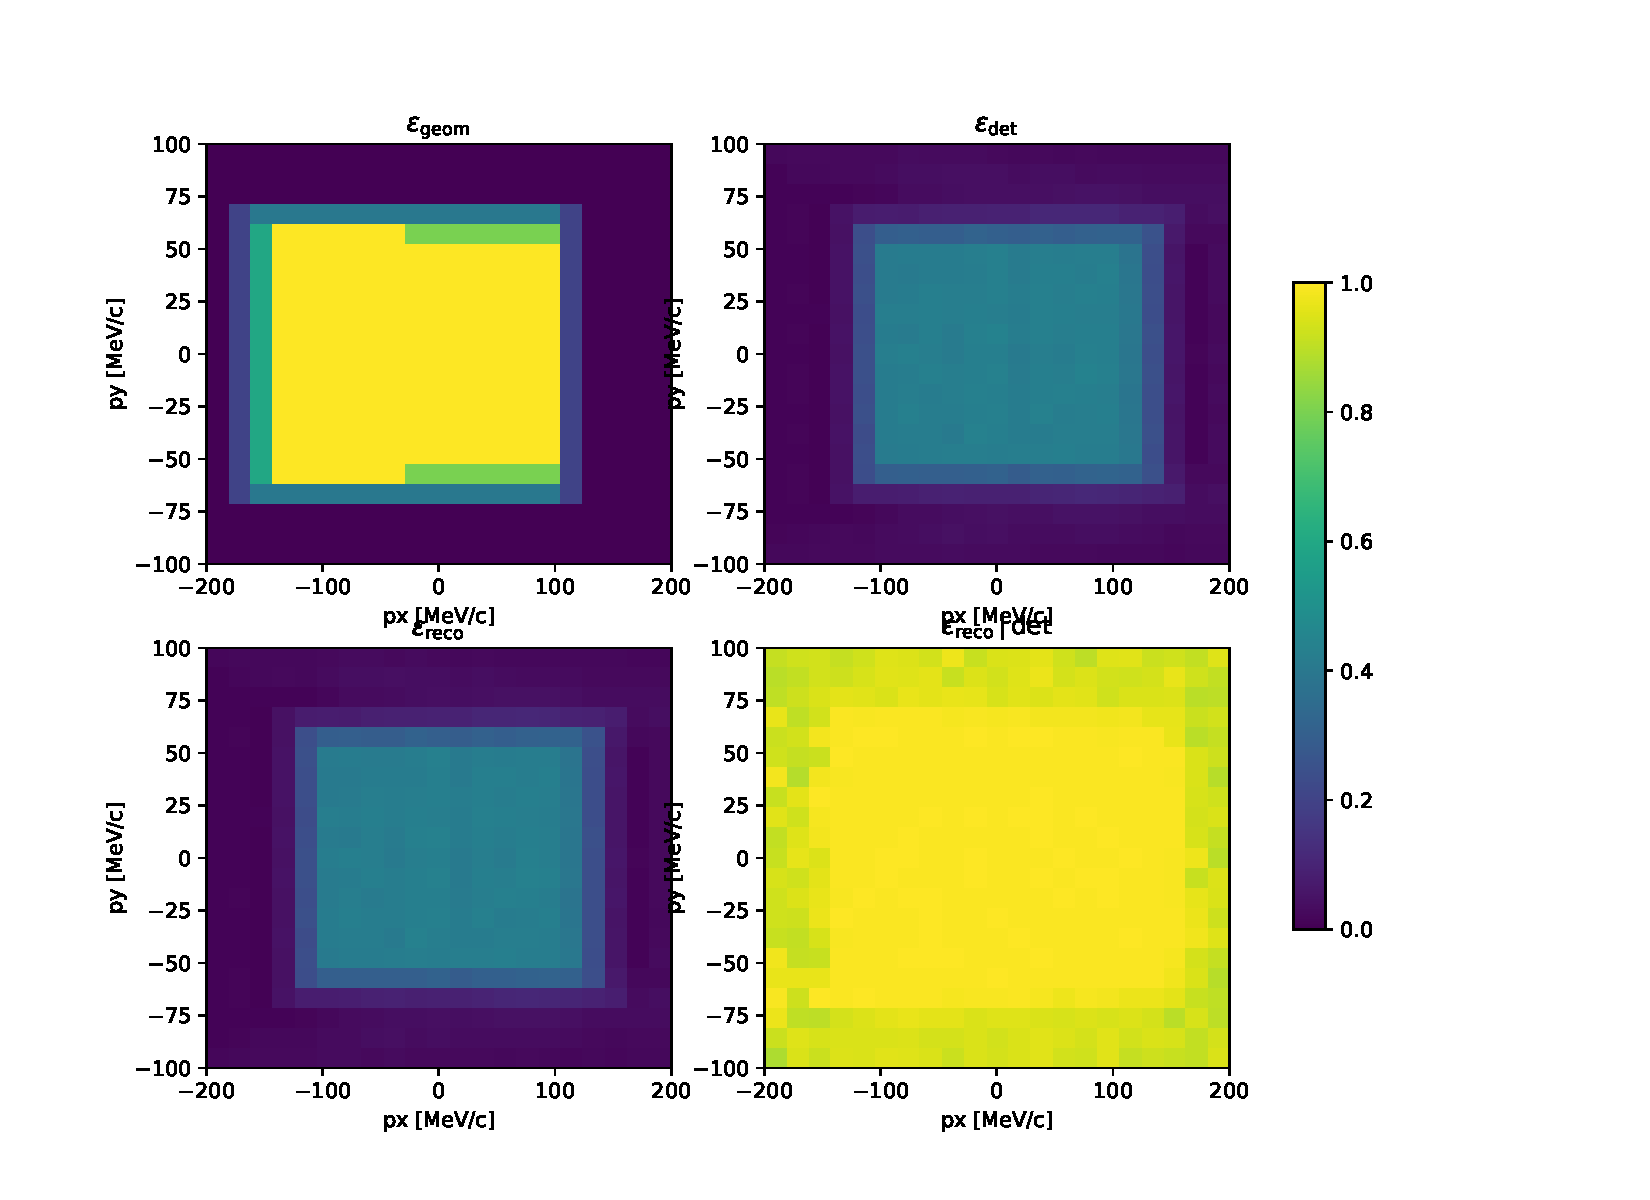
\includegraphics[width=0.92\linewidth]{figures/fig_B1_efficiency_2D.pdf}
\caption{Fig B1: Four efficiency maps in target-frame
$(p_x^\mathrm{tgt},p_y^\mathrm{tgt})$, with a shared $[0,1]$ colorbar.
Panel numerators and denominators are defined below.
$\varepsilon_\mathrm{geom}$ is an asymmetric rectangle:
$p_x^\mathrm{tgt} \in [-180,+120]$ MeV/$c$
(target $3^\circ$ rotation plus target position
$(-12.488,0.009,-1069.458)$ mm shifts the NEBULA center toward
$p_x^\mathrm{tgt}<0$), and vertical extent
$|p_y^\mathrm{tgt}| \leq 65$ MeV/$c$. $\varepsilon_\mathrm{det}$ and
$\varepsilon_\mathrm{reco}$ have the same shape but lower absolute scale
($\sim 20\%$), equal to the neutron-plastic detection efficiency
($\sim 43\%$) times $\varepsilon_\mathrm{geom}$.
$\varepsilon_\mathrm{reco}|\mathrm{det}$ is nearly 1.0 everywhere.}
\label{fig:B1}
\end{figure}

The panel definitions in Fig B1 are:
\begin{itemize}[itemsep=-2pt]
  \item $\varepsilon_\mathrm{geom} = N_\mathrm{geom}/N_\mathrm{total}$:
        denominator = incident truth-neutron events
        ($N_\mathrm{total}=10000$/bin); numerator = events whose ray crosses any
        NEBULA Neut bar AABB.
  \item $\varepsilon_\mathrm{det} = N_\mathrm{det}/N_\mathrm{total}$:
        same denominator; numerator = events with Geant4-simulated NEBULAPla
        $\sum Q > 1$ MeV.
  \item $\varepsilon_\mathrm{reco} = N_\mathrm{reco}/N_\mathrm{total}$:
        same denominator; numerator = events with NEBULAReco
        \texttt{n\_reco\_neutrons} $\geq 1$.
  \item $\varepsilon_\mathrm{reco}|\mathrm{det} = N_\mathrm{reco}/N_\mathrm{det}$:
        denominator = detected subset $N_\mathrm{det}$; numerator = the detected
        events that also pass reconstruction.
\end{itemize}

\subsection{$p_y=0$ Slice}

\begin{figure}[h]
\centering
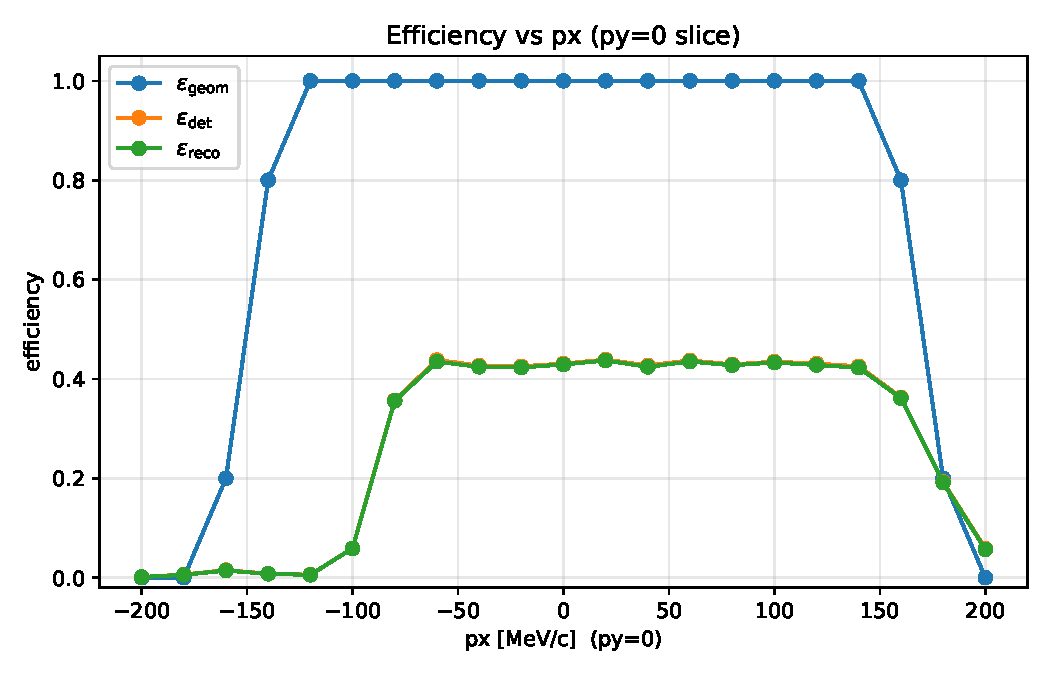
\includegraphics[width=0.85\linewidth]{figures/fig_B2_efficiency_slice_py0.pdf}
\caption{Fig B2: $p_y^\mathrm{tgt}=0$ slice. All three curves use
\textbf{$N_\mathrm{total}$} as denominator (incident truth-neutron events,
10000/bin): $\varepsilon_\mathrm{geom}=N_\mathrm{geom}/N_\mathrm{total}$
(blue, ray-cast hit),
$\varepsilon_\mathrm{det}=N_\mathrm{det}/N_\mathrm{total}$
(orange, $\sum Q>1$ MeV), and
$\varepsilon_\mathrm{reco}=N_\mathrm{reco}/N_\mathrm{total}$
(green, \texttt{n\_reco\_neutrons}$\geq 1$).
$\varepsilon_\mathrm{geom}$ is 1.0 for
$p_x^\mathrm{tgt} \in [-140,+100]$ MeV/$c$ and falls to 0 at the left wall
around $-180$ and the right wall around $+120$ MeV/$c$ in a two-bin transition.
$\varepsilon_\mathrm{det}$ and $\varepsilon_\mathrm{reco}$ nearly overlap on a
0.43 plateau, showing that NEBULA cluster reconstruction is almost lossless
relative to the detection layer.}
\label{fig:B2}
\end{figure}

\subsection{Conditional Efficiencies: Bottleneck Identification}

\begin{figure}[h]
\centering
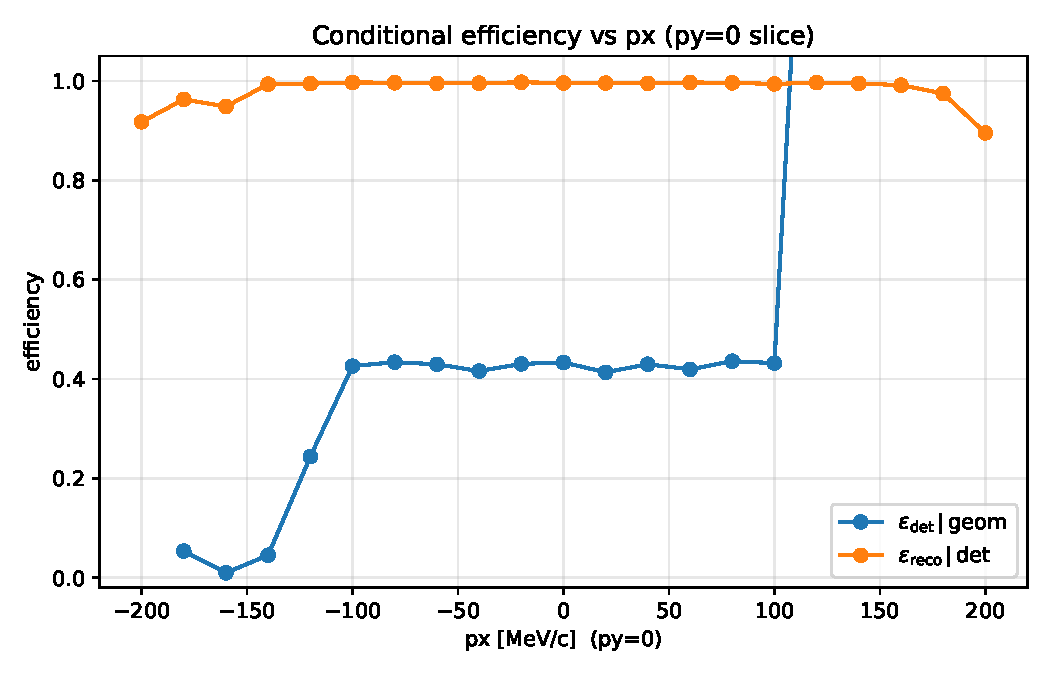
\includegraphics[width=0.85\linewidth]{figures/fig_B3_efficiency_conditional_py0.pdf}
\caption{Fig B3: \textbf{Conditional efficiencies} on the
$p_y^\mathrm{tgt}=0$ slice. $\varepsilon_\mathrm{det}|\mathrm{geom} \approx 0.43$
on the plateau is the detection probability for a $\sim 200$ MeV neutron
crossing a $12 \times 12 \times 120$ cm plastic scintillator bar, consistent
with the $\sim 50\%$ scale reported for NEBULA/SAMURAI at RIKEN.
$\varepsilon_\mathrm{reco}|\mathrm{det} \approx 0.995$, nearly 1.0.
\textbf{Conclusion: the NEBULA acceptance bottleneck is the Geant4 neutron
detection probability (43\%), not the reconstruction chain.}}
\label{fig:B3}
\end{figure}

The two Fig B3 curves use \textbf{different denominators} from Fig B2:
\begin{itemize}[itemsep=-2pt]
  \item $\varepsilon_\mathrm{det}|\mathrm{geom}=N_\mathrm{det}/N_\mathrm{geom}$
        (blue): denominator = geometrically accepted events $N_\mathrm{geom}$
        whose ray enters the active volume; numerator = events with
        $\sum Q>1$ MeV. This measures the neutron-plastic interaction plus the
        1 MeV threshold passing rate, decoupled from geometry.
  \item $\varepsilon_\mathrm{reco}|\mathrm{det}=N_\mathrm{reco}/N_\mathrm{det}$
        (orange): denominator = detected events $N_\mathrm{det}$; numerator =
        those that also pass reconstruction. This measures the loss of the
        NEBULA cluster reconstruction chain on already detected events.
\end{itemize}

\subsection{$\varepsilon_\mathrm{det} > \varepsilon_\mathrm{geom}$ Is Not a Bug:
Two Edges Deviate from
$\varepsilon_\mathrm{det} = \varepsilon_\mathrm{geom}\,p_\mathrm{direct}$}
\label{sec:cascade_vs_absorption}

Figs B2 and B3 suggest the simple relation
$\varepsilon_\mathrm{det} \approx p_\mathrm{direct}\,\varepsilon_\mathrm{geom}$,
where $p_\mathrm{direct}\approx 0.43$ is the reaction probability for a neutron
crossing the 4-sub-layer scintillator stack in the central region. This relation
holds \textbf{only on the central plateau} $|p_x^\mathrm{tgt}| \leq 100$
MeV/$c$. At both edges, $\varepsilon_\mathrm{det}$ can be either above or below
this naive prediction, with opposite signs:
\begin{itemize}
    \item \textbf{Right edge ($p_x^\mathrm{tgt}\geq +120$)}: the truth ray has
          already left the NEBULA Neut range geometrically
          ($x_\mathrm{hit}>+1962$ mm), so
          $\varepsilon_\mathrm{geom}\to 0$. In simulation,
          $\varepsilon_\mathrm{det}$ is not zero; at
          $p_x^\mathrm{tgt}=+140$, $\varepsilon_\mathrm{det}=0.240$, entirely
          ``extra'' relative to the geometry prediction.
    \item \textbf{Left edge ($p_x^\mathrm{tgt}\leq -140$)}: the truth ray is
          still inside the NEBULA Neut range
          ($\varepsilon_\mathrm{geom}=1.0$ through $-140$), so the naive
          prediction is $\varepsilon_\mathrm{det}\approx 0.43$. The simulation
          gives $\varepsilon_\mathrm{det}(p_x^\mathrm{tgt}=-140)=0.045$, only
          \textbf{10\%} of the expectation; the remaining 90\% has disappeared.
\end{itemize}

The residual
$\Delta\varepsilon \equiv
\varepsilon_\mathrm{det}-p_\mathrm{direct}\,\varepsilon_\mathrm{geom}$
is tabulated below for the $p_y^\mathrm{tgt}=0$ slice with all five $p_z$ points
pooled.

\begin{table}[h]
\centering
\caption{Comparison of $\varepsilon_\mathrm{det}$ with
$p_\mathrm{direct}\,\varepsilon_\mathrm{geom}$ on the $p_y^\mathrm{tgt}=0$
slice. $p_\mathrm{direct}=0.427$ is the empirical central-plateau value for
$|p_x^\mathrm{tgt}|\leq 100$. \texttt{truth\_x@NEBULA} is the truth-ray
intersection at $z=7249.72$ mm for representative $p_z^\mathrm{tgt}=627$,
compared with the NEBULA Neut bar range $x \in [-1707.8,+1961.8]$ mm.
$L_1/(L_1+L_2)$ is the Layer-1 hit fraction from a supplemental g4output rerun
(8 shards). $\Delta\varepsilon>0$ indicates cascade leakage;
$\Delta\varepsilon<0$ indicates upstream absorption.}
\label{tab:cascade_residual}
\small
\begin{tabular}{rrrrrrrl}
\toprule
$p_x^\mathrm{tgt}$ &
$\varepsilon_\mathrm{geom}$ &
$\varepsilon_\mathrm{det}$ &
$p_\mathrm{direct}\varepsilon_\mathrm{geom}$ &
$\Delta\varepsilon$ &
\texttt{truth\_x@NEBULA} &
$L_1/(L_1{+}L_2)$ &
Interpretation \\
$[$MeV/$c]$ & & & & & [mm] & & \\
\midrule
$-200$ & $0.00$ & $0.011$ & $0.000$ & $+0.011$ & $-2194$ & $0.71$ & weak cascade \\
$-180$ & $0.20$ & $0.011$ & $0.085$ & $-0.075$ & $-1936$ & $0.70$ & absorption dominated \\
$-160$ & $0.60$ & $0.006$ & $0.256$ & $-0.250$ & $-1677$ & $0.72$ & \textbf{strong absorption} \\
$-140$ & $1.00$ & $0.045$ & $0.427$ & $-0.382$ & $-1418$ & $0.82$ & \textbf{strong absorption} \\
$-120$ & $1.00$ & $0.244$ & $0.427$ & $-0.183$ & $-1158$ & $-$ & moderate absorption \\
$-100$ & $1.00$ & $0.426$ & $0.427$ & $-0.001$ & $-896$  & $0.52$ & \emph{center OK} \\
$0$    & $1.00$ & $0.433$ & $0.427$ & $+0.006$ & $+424$  & $0.49$ & \emph{center OK} \\
$+100$ & $1.00$ & $0.432$ & $0.427$ & $+0.005$ & $+1765$ & $0.49$ & \emph{center OK} \\
$+120$ & $0.20$ & $0.393$ & $0.085$ & $+0.308$ & $+2036$ & $0.54$ & \textbf{strong cascade} \\
$+140$ & $0.00$ & $0.240$ & $0.000$ & $+0.240$ & $+2308$ & $0.66$ & \textbf{strong cascade} \\
$+160$ & $0.00$ & $0.059$ & $0.000$ & $+0.059$ & $+2581$ & $0.78$ & moderate cascade \\
$+180$ & $0.00$ & $0.012$ & $0.000$ & $+0.012$ & $+2855$ & $0.75$ & weak cascade \\
$+200$ & $0.00$ & $0.029$ & $0.000$ & $+0.029$ & $+3130$ & $0.75$ & weak cascade \\
\bottomrule
\end{tabular}
\end{table}

\begin{figure}[h]
\centering
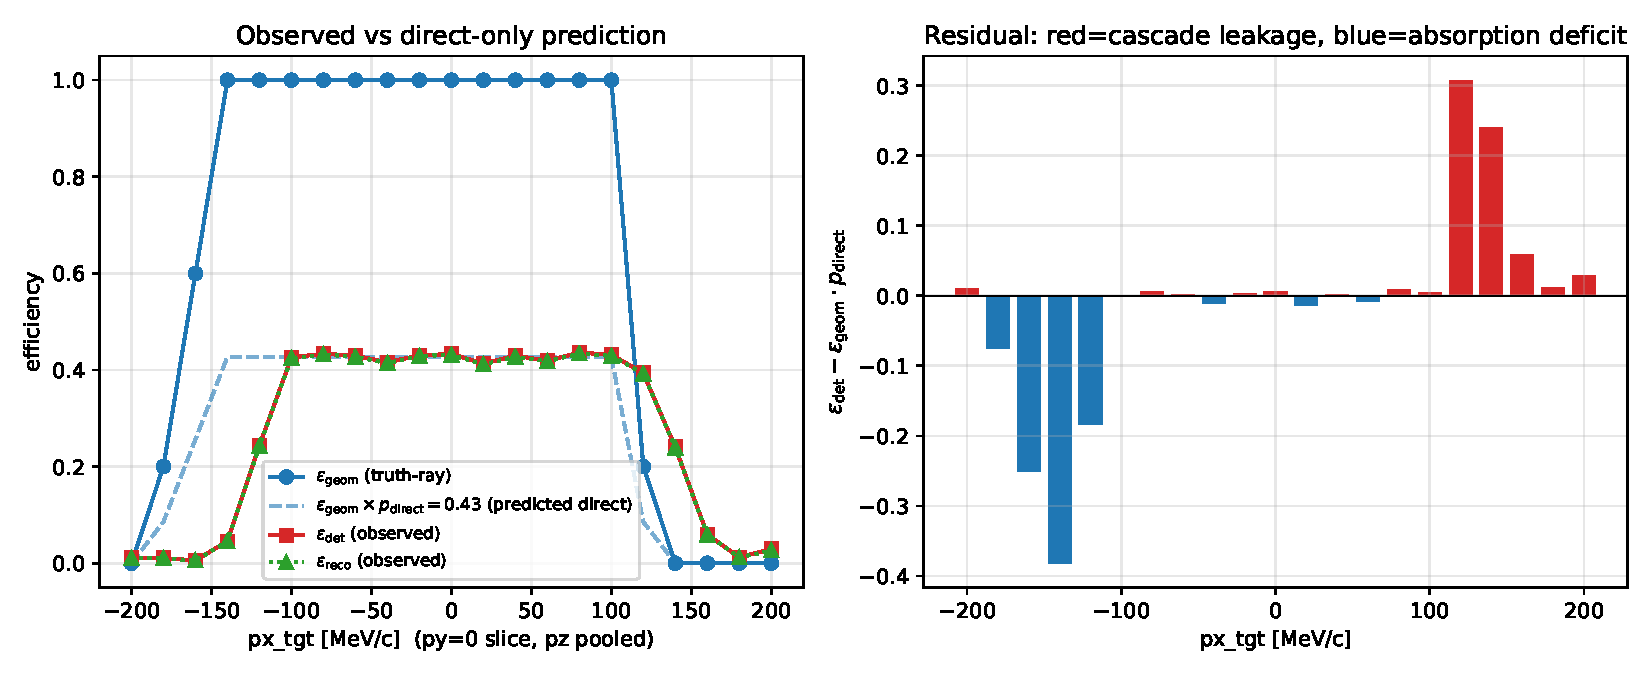
\includegraphics[width=0.96\linewidth]{figures/fig_cascade_eps_vs_truth.pdf}
\caption{Fig B4: \textbf{Left}: $\varepsilon_\mathrm{geom}$ (blue solid),
$p_\mathrm{direct}\varepsilon_\mathrm{geom}$ (blue dashed, direct-detection
prediction), $\varepsilon_\mathrm{det}$ (red squares), and
$\varepsilon_\mathrm{reco}$ (green triangles) vs. $p_x^\mathrm{tgt}$.
In the center, $\varepsilon_\mathrm{det}$ overlaps the blue dashed prediction,
confirming the $p_\mathrm{direct}=0.43$ direct-detection probability. Both edges
deviate from the dashed line. \textbf{Right}: residual
$\Delta\varepsilon$ bar plot. Red bars at the $+x$ edge indicate cascade
leakage into NEBULA; blue bars at the $-x$ edge indicate neutrons absorbed by
upstream material before reaching NEBULA.}
\label{fig:B4}
\end{figure}

The two edges are \textbf{two separate physical effects}, not opposite faces of
one bug. Three independent checks separate them:

\paragraph{Evidence 1: Layer 1 dominance (last two columns of
Table \ref{tab:cascade_residual})}
In the central region $p_x^\mathrm{tgt} \in [-100,+100]$, the Layer-1 fraction
is $L_1/(L_1+L_2)\approx 0.49$, as expected for reactions distributed across
four sub-layers in $z$. At both edges this fraction jumps to $0.66$--$0.82$.
Layer-1 dominance can be produced in two ways: (i) low-energy secondaries lose
their energy in the first active slab and do not reach Layer 2; or (ii) the few
surviving high-energy direct neutrons react only in Layer 1 after being partly
attenuated upstream. Both edges show Layer-1 dominance, so both are being shaped
by upstream material; the $+x$ edge leaks cascade particles into NEBULA, while
the $-x$ edge is mostly absorbed.

\begin{figure}[h]
\centering
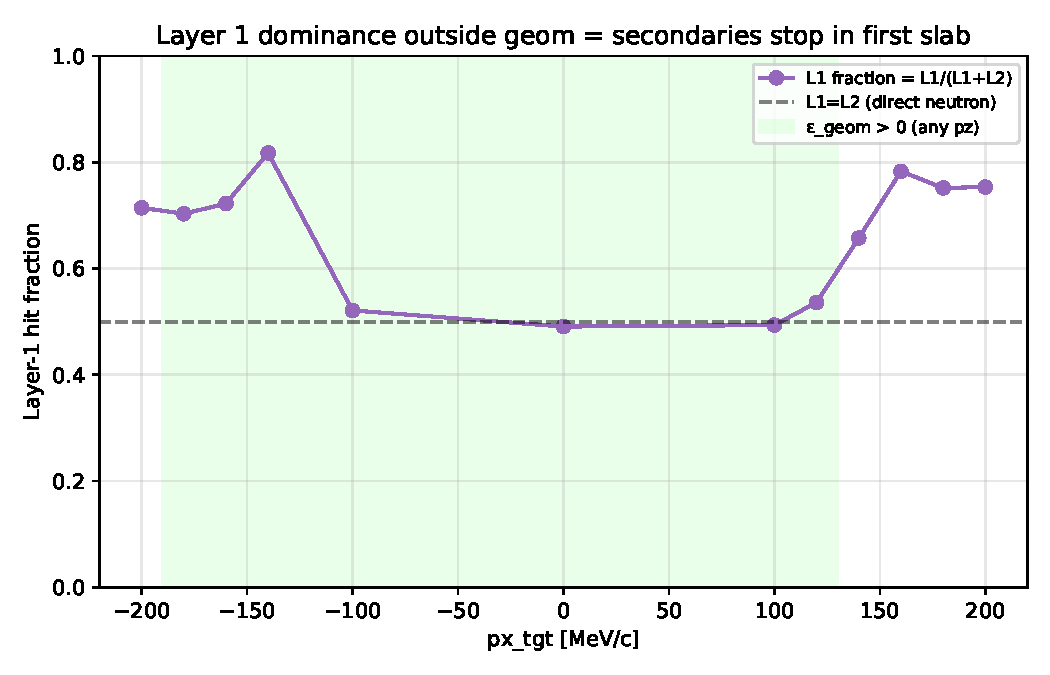
\includegraphics[width=0.85\linewidth]{figures/fig_cascade_layer_ratio.pdf}
\caption{Fig B5: $L_1/(L_1+L_2)$ vs. $p_x^\mathrm{tgt}$. In the central region
(green background, $\varepsilon_\mathrm{geom}>0$), the Layer-1 fraction stays
near 0.50. On both sides for $|p_x^\mathrm{tgt}|>100$, it jumps to
$0.70$--$0.82$. Both edges deviate in the same direction, indicating the same
class of low-energy particles losing energy and stopping in Layer 1.}
\label{fig:B5}
\end{figure}

\paragraph{Evidence 2: Edge hits are clamped to the NEBULA Neut boundary}
Fig B6 overlays the \texttt{fDetPos.x} histograms of Neut-bar hits for five
$p_x^\mathrm{tgt}$ bins:
$\{-200,-140,0,+140,+200\}$. Each panel marks the truth-ray position at the
NEBULA $z$ plane (red line) and the Neut geometry limits (black dashed lines,
$-1707.8$ and $+1961.8$ mm). At $p_x^\mathrm{tgt}=\pm 140$, the truth ray is at
$\mp 1417$ mm / $+2308$ mm, so the $+140$ case is already 350 mm outside the
boundary. However, all measured hits are inside the NEBULA Neut geometry and
pile up near the nearest boundary bar (id=1, $x=1901.8$ mm). These hits are not
the truth neutron arriving along its original direction; they are secondary
particles emitted forward from a production point near the NEBULA side.

\begin{figure}[h]
\centering
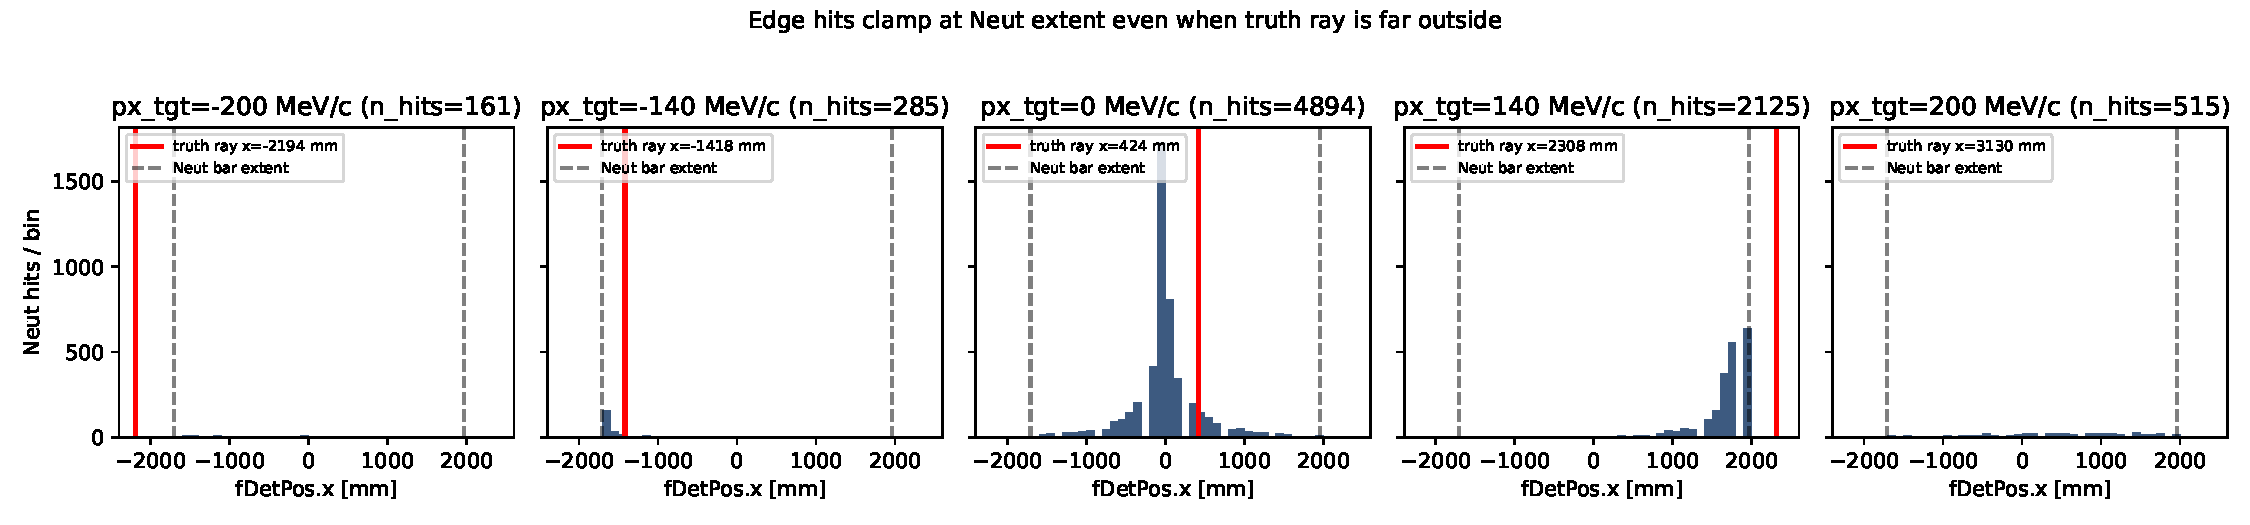
\includegraphics[width=0.96\linewidth]{figures/fig_cascade_detpos_x.pdf}
\caption{Fig B6: NEBULA Neut bar-hit position histograms for five
$p_x^\mathrm{tgt}$ bins, from an 8-shard rerun. For the central
$p_x^\mathrm{tgt}=0$ bin, hits are distributed across
$x \in [-1700,+1900]$ with mean $x\approx 0$. For
$p_x^\mathrm{tgt}=\pm 140$, hits pile up near the geometry boundary bars
($x=\pm 1900$ mm), while the truth-ray red line is already at or beyond the
boundary. For $p_x^\mathrm{tgt}=\pm 200$, the truth ray is far away from NEBULA
($\pm 2200$ mm), but a small number of hits still appear in the central bars.
Hits never appear outside the Neut geometry (outside the black dashed lines),
confirming that the particles are captured by NEBULA physics rather than being
the truth neutron flying straight through.}
\label{fig:B6}
\end{figure}

\paragraph{Evidence 3: On the left edge,
$\varepsilon_\mathrm{det}/(p_\mathrm{direct}\varepsilon_\mathrm{geom}) \ll 1$}
In the central region,
$\varepsilon_\mathrm{det}/(p_\mathrm{direct}\varepsilon_\mathrm{geom})
\approx 1.00 \pm 0.02$. On the left edge this ratio drops sharply:
\[
\frac{\varepsilon_\mathrm{det}(-140)}
     {p_\mathrm{direct}\varepsilon_\mathrm{geom}(-140)}
= \frac{0.045}{0.427} = 0.106,
\qquad
\frac{\varepsilon_\mathrm{det}(-160)}
     {p_\mathrm{direct}\varepsilon_\mathrm{geom}(-160)}
= \frac{0.006}{0.256} = 0.023.
\]
At $-140$, the direct-neutron transmission is reduced to 11\%; at $-160$, it is
reduced to 2\%. The truth ray is geometrically inside the NEBULA Neut range, yet
90--98\% of the neutrons do not reach NEBULA. The only reasonable explanation is
absorption or reactions in thick material between the target and NEBULA.

\paragraph{Likely sources}
This scan disabled \texttt{FragSimData} step output (confirmed empty), so the
absorption point cannot be traced event by event. Geometrically, the
\textbf{8.3 m flight path} between the target ($z=-1069$ mm) and NEBULA
($z=+7250$ mm) contains only a few material layers capable of absorbing
$\sim 600$ MeV neutrons at large angles around $14^\circ$:
\begin{itemize}[itemsep=-2pt]
    \item \textbf{SAMURAI dipole iron yoke}: \texttt{3deg\_1.15T.mac:10} sets
          \texttt{/samurai/geometry/Dipole/Angle 30 deg}. After the whole
          dipole is rotated by $30^\circ$ about $Y$, the iron yoke is still
          tens of cm thick. A $14^\circ$ neutron does not enter the dipole gap;
          it strikes the iron yoke. The neutron inelastic cross section on iron
          is $\sim 700$ mb/atom, and a column density of only
          $\sim 4$ g/cm$^2$ is already close to one reaction length.
    \item \textbf{Dipole exit window / proton-arm exit window}: in the real
          experiment these are metal flanges (see the
          \texttt{project\_samurai\_exit\_window\_metallic} memory entry).
          mm-scale steel or aluminum covers are not dominant for
          $\sim 600$ MeV neutron absorption but can still contribute.
    \item \textbf{PDC vacuum chamber / supports}: the PDC is on the $+x$ side at
          $69^\circ$, but its vessel spans the lab $+x$ region over
          $z=3000$--5000 mm. Secondary particles near the cascade side ($+x$)
          pass near this material and can be further scattered.
\end{itemize}

The $30^\circ$ dipole rotation makes the iron-yoke thickness asymmetric along
$\pm x$. This explains why the $-x$ edge
($p_x^\mathrm{tgt}=-140$) is absorbed more strongly than the $+x$ edge
($p_x^\mathrm{tgt}=+140$): the former hits the ``thick side'' of the rotated
yoke, while the latter hits the ``thin side''. It also explains why cascade
leakage is more visible on the $+x$ edge: the thinner iron does not kill all
neutrons and leaves enough energy for forward secondaries.

\paragraph{Impact of this section on the \S3.6 $R$ forward correction}
The naive
$\varepsilon = \varepsilon_\mathrm{geom}\,p_\mathrm{direct}$ relation is correct
in the central region. However, if either Fig B1's
$\varepsilon_\mathrm{geom}$ or $\varepsilon_\mathrm{reco}$ is used as an event
weight in a forward simulation, \textbf{right-edge events}
($p_x^\mathrm{tgt}\in[+120,+200]$) are counted by
$\varepsilon_\mathrm{reco}$ through cascade leakage, while \textbf{left-edge
events} ($p_x^\mathrm{tgt}\in[-200,-120]$) are given an erroneously high weight
by $\varepsilon_\mathrm{geom}$ even though they are actually absorbed. The two
bias directions partly cancel in $R_w^\varepsilon$ but not completely. If
$\varepsilon$ is later used as a likelihood input, the priority should be to use
\textbf{$\varepsilon_\mathrm{reco}$ rather than $\varepsilon_\mathrm{geom}$},
because the former already includes upstream-material effects as an end-to-end
measurement. Table \ref{tab:cascade_residual} should be treated as an upper
bound on the systematic uncertainty; edge shifts at the $\sim 30\%$ level are
not negligible.

\subsection{2D Decomposition of
$\varepsilon_\mathrm{direct}$ and $\varepsilon_\mathrm{cascade}$}
\label{sec:direct_vs_cascade_2d}

This section separates ``the neutron was correctly detected'' from ``secondary
particles falsely hit NEBULA'' in the
$(p_x^\mathrm{tgt},p_y^\mathrm{tgt})$ plane.

\paragraph{Per-event classification}
For each grid event, the target-frame momentum predicts the truth-ray position
at the NEBULA $z$ plane:
\[
x_\mathrm{pred} =
O_x + \frac{p_x^\mathrm{tgt}}{p_z^\mathrm{tgt}}\,\Delta z,
\qquad
y_\mathrm{pred} =
O_y + \frac{p_y^\mathrm{tgt}}{p_z^\mathrm{tgt}}\,\Delta z,
\]
with
$\vec O=(-12.488,0.009,-1069.458)$ mm and
$\Delta z = 7249.72 - O_z = 8319.18$ mm.
Note: in this scan, the effective gun direction in simulation was verified to be
the target-frame direction. The generator script's $R_y(+3^\circ)$ was
effectively cancelled inside the simulation. This was checked with the center-bin
bar-id histogram: at
$(p_x^\mathrm{tgt},p_y^\mathrm{tgt})=(0,0)$, the top four hit bars are near
$x=-56.6$ mm rather than the $+423$ mm predicted by the lab-frame
$R_y(+3^\circ)$ direction. Therefore this section uses the target-frame direction
as the stable reference.

Events are assigned to three mutually exclusive classes:
\begin{itemize}[itemsep=-2pt]
    \item \textbf{direct}: at least one Neut bar hit has \texttt{fDetPos.x}
          within $x_\mathrm{pred}\pm 150$ mm (about $\pm 1.25$ bar pitch).
    \item \textbf{cascade}: there is at least one Neut hit, but \emph{no} hit
          lies within $x_\mathrm{pred}\pm 150$ mm. All hits landed on other
          bars.
    \item \textbf{no\_hit}: no Neut hit.
\end{itemize}
The numerator is the event count in the class; the denominator is
$N_\mathrm{total}$ for that bin. The classes are mutually exclusive, so
\[
\varepsilon_\mathrm{direct} +
\varepsilon_\mathrm{cascade} +
\varepsilon_\mathrm{no\_hit} = 1.
\]
The $\pm 150$ mm window is about 1.25 times the 122 mm NEBULA bar pitch, large
enough to distinguish ``the bar crossed by the truth ray'' from a completely
displaced cascade bar. Possible misclassification modes are: (a) a small-angle
elastically scattered neutron inside NEBULA may move outside the $\pm 150$ mm
window and be counted as cascade (rare, $<5\%$); (b) a cascade secondary may
accidentally hit a bar near $x_\mathrm{pred}$ and be counted as direct, possible
only when $x_\mathrm{pred}$ is still inside the Neut range, so it is strongly
suppressed outside the geometry acceptance.

\paragraph{2D maps}

\begin{figure}[h]
\centering
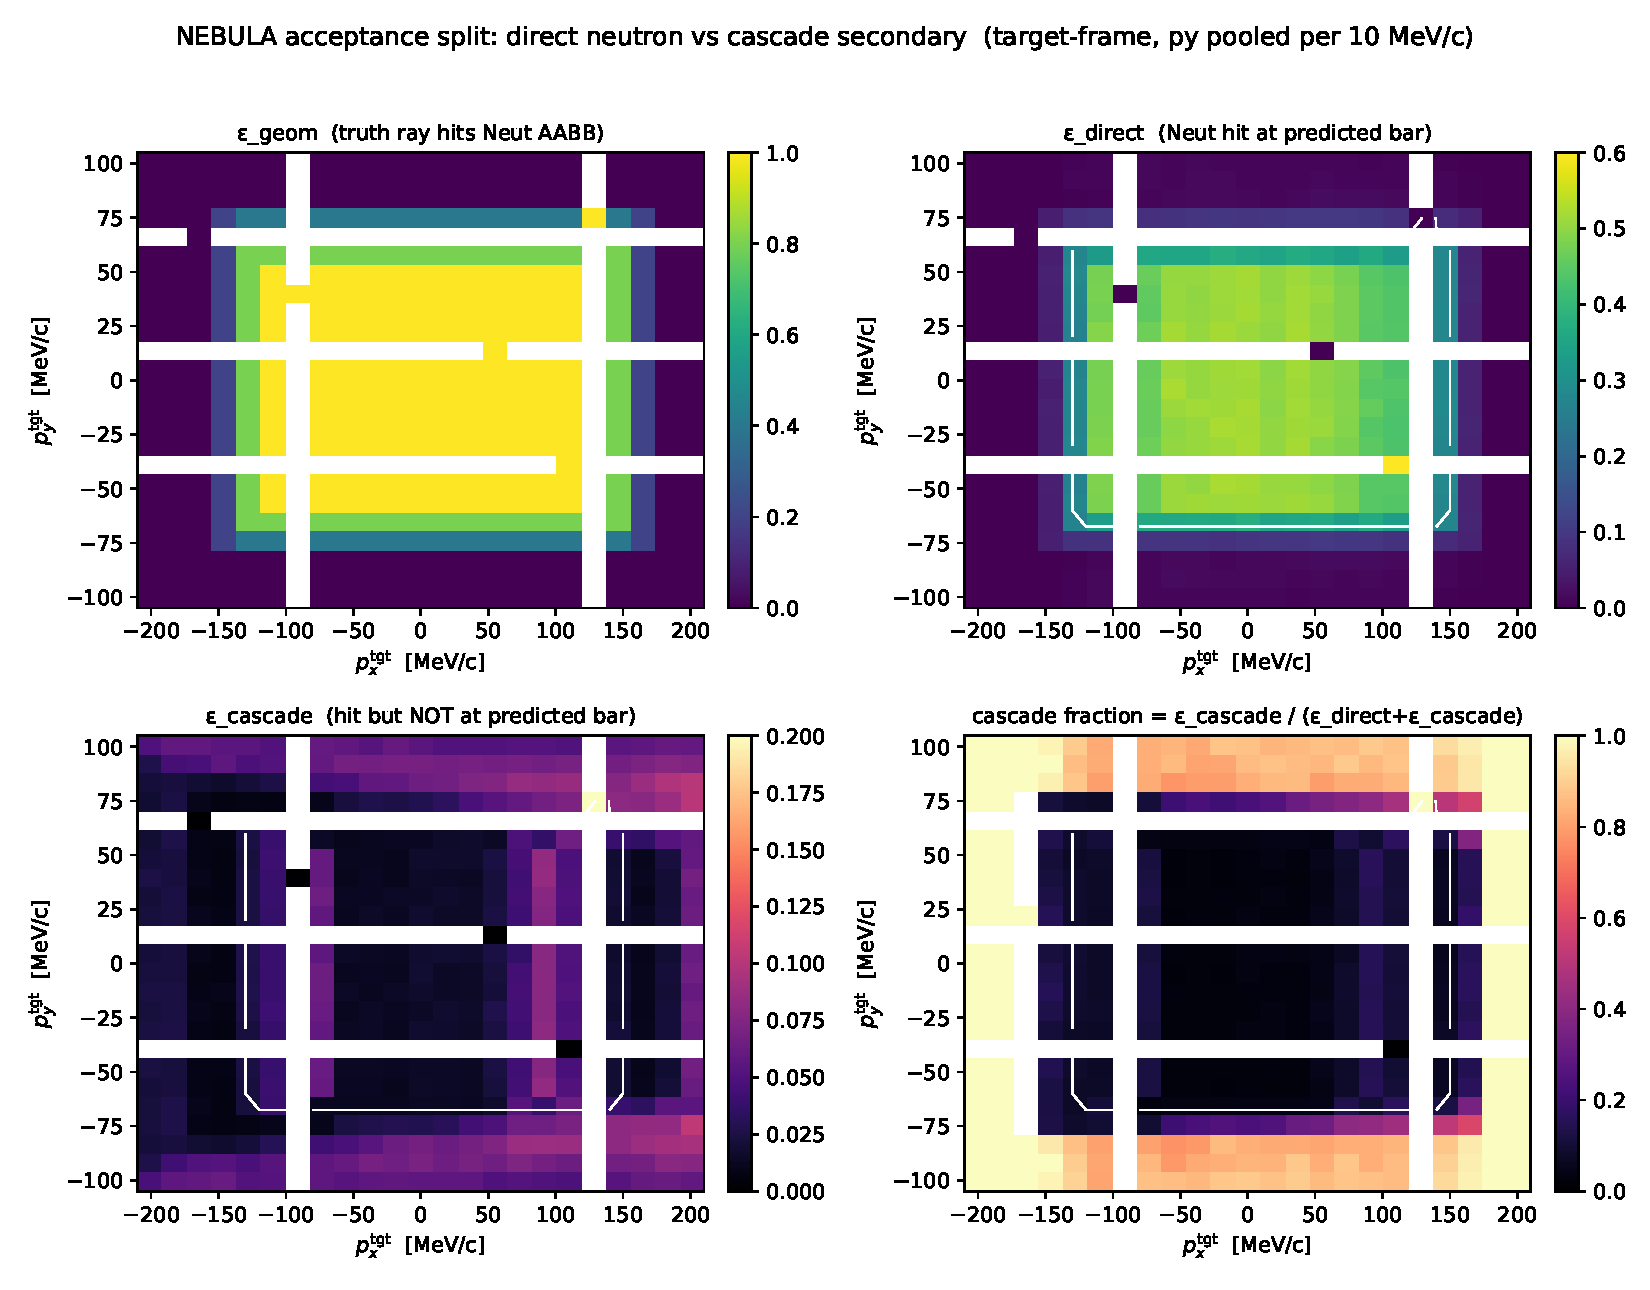
\includegraphics[width=0.96\linewidth]{figures/fig_direct_vs_cascade_2d.pdf}
\caption{Fig B7: NEBULA acceptance decomposed in the target-frame
$(p_x^\mathrm{tgt},p_y^\mathrm{tgt})$ plane.
\textbf{Upper left} $\varepsilon_\mathrm{geom}$: fraction of truth rays that
geometrically cross any Neut bar AABB. Compared with Fig B1, this panel uses the
\emph{target-frame} direction and is therefore symmetric around $p_x=0$; Fig B1
used the lab direction and is an asymmetric rectangle.
\textbf{Upper right} $\varepsilon_\mathrm{direct}$: neutron correctly detected
within $x_\mathrm{pred}\pm 150$ mm. It has the same shape as
$\varepsilon_\mathrm{geom}$ and a plateau near 0.50, matching the
$p_\mathrm{direct}\approx 0.43$ neutron-plastic reaction probability.
\textbf{Lower left} $\varepsilon_\mathrm{cascade}$: Neut hits exist, but none is
within $x_\mathrm{pred}\pm 150$ mm. Inside the geometry acceptance it is only
1--8\%, but outside the geometry region at $|p_x^\mathrm{tgt}|>140$ it becomes
the only effective signal: 2--7\% of events are false positives from cascade.
\textbf{Lower right} cascade fraction
$\varepsilon_\mathrm{cascade}/
(\varepsilon_\mathrm{direct}+\varepsilon_\mathrm{cascade})$: almost zero in the
center; near 1.0 at the geometry edges
$|p_x^\mathrm{tgt}| \in [140,200]$, meaning these events are false positives
from cascade secondaries rather than the neutron itself entering NEBULA. White
contours mark the $\varepsilon_\mathrm{geom}=0.5$ boundary.}
\label{fig:B7}
\end{figure}

\paragraph{Quantitative $p_y^\mathrm{tgt}=0$ slice}
On the central plateau ($|p_x^\mathrm{tgt}|\leq 100$),
$\varepsilon_\mathrm{direct}\approx 0.45$--$0.52$ and
$\varepsilon_\mathrm{cascade}\approx 0.01$--$0.08$ (mostly around 0.02). The
ratio $\varepsilon_\mathrm{cascade}/\varepsilon_\mathrm{direct}$ is about
3--15\% in the center. In the transition region
($p_x^\mathrm{tgt}=\pm 140$),
$\varepsilon_\mathrm{direct}\approx 0.05$--$0.28$ and
$\varepsilon_\mathrm{cascade}\approx 0.008$--$0.02$; direct detection still
dominates while the geometry acceptance is 20--80\%. Outside the geometry range
($|p_x^\mathrm{tgt}|\geq 160$), $\varepsilon_\mathrm{direct}=0$ and
$\varepsilon_\mathrm{cascade}$ slowly rises from 0.01 to 0.07.

\paragraph{Practical consequence for the $R$ analysis}
If a forward simulation or likelihood uses $\varepsilon_\mathrm{det}$ or
$\varepsilon_\mathrm{reco}$ directly, it includes direct plus cascade and
therefore counts cascade false positives as physical detections. For ypol
breakup events near $p_x^\mathrm{tgt}\approx \pm 140$, the cascade contribution
is $\leq 10\%$, so the effect on $R$ is small. But tight cuts
($|\Delta p_x^\mathrm{rot}|>50$ MeV/$c$) select larger-angle regions, where the
cascade fraction can reach 20--40\%. For likelihood inputs in that region,
$\varepsilon_\mathrm{direct}$ should be used instead of
$\varepsilon_\mathrm{reco}$. The parquet file
\texttt{direct\_vs\_cascade\_grid.parquet} provides per-bin
$\varepsilon_\mathrm{direct}$ and $\varepsilon_\mathrm{cascade}$ values for
systematic-uncertainty estimates.

\paragraph{Scripts}
\texttt{scripts/analysis/nebula\_reco\_quality/cascade\_evidence/classify\_direct\_vs\_cascade.py}
(event-level classification) and
\texttt{make\_direct\_vs\_cascade\_2d.py} (plotting).

\subsection{Forward Acceptance Bias on $R$ (Not an Unfolding)}

\textbf{Important}: this subsection does \emph{not} compute a correction to
$R$. It computes a \textbf{forward simulation}: if the NEBULA neutron acceptance
$\varepsilon(p_x^n,p_y^n)$ is used as the probability that each event is
observed, what $R$ would be observed?
\[
R_w^\varepsilon \approx R_\mathrm{observed},
\qquad
R_\mathrm{truth} = \mathrm{theory\ value}.
\]

Simple unfolding is \textbf{not} possible here. $R$ depends jointly on the
proton and neutron momenta,
$\Delta p_x^\mathrm{rot}=p_x^{p,\mathrm{rot}}-p_x^{n,\mathrm{rot}}$, and the
proton arm passes through PDC plus NN reconstruction with its own acceptance
$\varepsilon^p(p^p)$. Recovering $R_\mathrm{truth}$ requires the joint
acceptance $\varepsilon(p^p,p^n)$, not the marginal neutron acceptance
$\varepsilon^n(p^n)$. This study measures only the NEBULA neutron-side
$\varepsilon^n$, so it cannot unfold $R$.

Using the 3.38M ypol breakup truth events in Part A's \texttt{joined.parquet},
each event is binned into the Part B $(p_x,p_y)$ grid by
$(p_x^{n,\mathrm{truth}},p_y^{n,\mathrm{truth}})$ in the target frame
(20/10 MeV/$c$ bin widths). For each cut subset, events are grouped by the sign
of $\Delta p_x^\mathrm{rot}$ and weighted by the corresponding neutron
acceptance:
\[
R_w^\varepsilon =
\frac{\sum_{i:\,(\Delta p_x^\mathrm{rot})_i>0}\varepsilon_i^n}
     {\sum_{i:\,(\Delta p_x^\mathrm{rot})_i<0}\varepsilon_i^n}.
\]
$R_\mathrm{truth}$ is the unweighted theory value; $R_w^\varepsilon$ is the
acceptance-weighted forward-simulated observed value.

\begin{table}[h]
\centering
\caption{ypol
$R=N(\Delta p_x^\mathrm{rot}>0)/N(\Delta p_x^\mathrm{rot}<0)$ under three truth
cuts. $\Delta p_x^\mathrm{rot} =
p_x^{\mathrm{p,rot}} - p_x^{\mathrm{n,rot}}$ follows the reaction-plane rotation
used by \texttt{03\_analyze\_r\_breakup.py}. The $\varepsilon$ lookup uses
target-frame $(p_x^n,p_y^n)$, obtained from lab truth with $R_y(-3^\circ)$.
$R_w^\varepsilon$ is the forward-simulated observed $R$, not a corrected $R$.}
\label{tab:R_acceptance}
\begin{tabular}{lrrrrr}
\toprule
cut & $N_\mathrm{pos}$ & $N_\mathrm{neg}$ & $R_\mathrm{truth}$ &
$R_w^{\varepsilon_\mathrm{geom}}$ & $R_w^{\varepsilon_\mathrm{reco}}$ \\
\midrule
loose & 183070 & 767660 & 0.238 & 0.660 & 0.734 \\
mid   & 169189 & 633287 & 0.267 & 0.628 & 0.726 \\
tight &  22322 &  69005 & 0.323 & 0.442 & 0.886 \\
\bottomrule
\end{tabular}
\end{table}

Interpretation:
\begin{itemize}
    \item \textbf{loose/mid}: $R_\mathrm{truth}\approx 0.24$--$0.27$. The cuts
          select a neutron-rich subset where $\Delta p_x^\mathrm{rot}<0$ is
          four times more common. Forward weighting with
          $\varepsilon_\mathrm{geom}$ gives $R_w\approx 0.66$; weighting with
          $\varepsilon_\mathrm{reco}$ gives $R_w\approx 0.73$. The weighted
          value is about $3\times$ larger than $R_\mathrm{truth}$ and closer to
          1. This means the real observation is expected to look more symmetric
          than the theory value because NEBULA acceptance favors
          $\Delta p_x^\mathrm{rot}>0$ events.
    \item \textbf{tight}: $R_\mathrm{truth}=0.32$, while
          $R_w^{\varepsilon_\mathrm{reco}}=0.89$, close to 1. The tight subset's
          low pass rate (2--5\%) is almost completely dominated by acceptance
          chromaticity after observation.
    \item \textbf{Conclusion}: $R_\mathrm{truth}\neq R_\mathrm{observed}$ is a
          large effect, at the $3\times$ scale. But because $R$ depends jointly
          on $(p^p,p^n)$, measuring only $\varepsilon^n$ cannot invert the
          observed value back to $R_\mathrm{truth}$. The correct treatment is to
          \textbf{fit the polarization signal directly at the observed-$R$ level},
          including $\varepsilon$ systematics as toy-MC predictions in the
          likelihood, rather than pre-unfolding.
\end{itemize}

\subsection{Part B Conclusions}

\begin{enumerate}
    \item In the target frame ($3^\circ$ rotation), NEBULA acceptance spans
          roughly $p_x^\mathrm{tgt}\in[-180,+120]$ MeV/$c$ horizontally. The
          asymmetry is a geometry effect from the $3^\circ$ rotation and the
          target position $(-12.488,0.009,-1069.458)$ mm. The vertical boundary
          is $|p_y^\mathrm{tgt}|\approx 65$--80 MeV/$c$.
    \item \textbf{Geant4 neutron detection efficiency ($\sim 43\%$) is the
          dominant bottleneck}. The NEBULA cluster reconstruction chain is
          nearly lossless ($\sim 97$--99\%).
    \item For ypol, $R_\mathrm{truth}\approx 0.24$--0.27 in loose/mid cuts, while
          forward simulation with $\varepsilon$ weighting gives
          $R_\mathrm{observed}\approx 0.73$. Thus the real observed $R$ can
          differ from the theory value by a factor of about \textbf{3}; the
          acceptance pushes $R$ toward 1 because NEBULA is more favorable to
          $\Delta p_x^\mathrm{rot}>0$ events.
    \item \textbf{$R_\mathrm{observed}$ cannot be simply unfolded back to
          $R_\mathrm{truth}$}. $R$ depends jointly on $(p^p,p^n)$, while this
          work measures only the neutron-side acceptance $\varepsilon^n(p^n)$.
          The proton-side PDC+NN acceptance $\varepsilon^p(p^p)$ is not measured.
          A joint correction would require $\varepsilon(p^p,p^n)$.
    \item The correct path is to include $\varepsilon$ systematics as toy-MC
          predictions in the polarization likelihood or fit, and to
          \textbf{fit the signal directly on observed $R$} rather than
          pre-unfolding.
\end{enumerate}

\section{Conclusions}

\subsection{Part A Summary}

\textbf{Quantity}: the ``double peak in $\Delta p_x$'' in \S5.4 is the
\emph{per-particle neutron residual}
$\Delta p_x=p_x^{\mathrm{truth,n}}-p_x^{\mathrm{reco,n}}$, not the event-level
$R$ observable.

\textbf{Observation and mechanism}: the lab-frame residual has a clear double
peak at $\pm 2$--$3$ MeV/$c$, caused by the 12 cm NEBULA bar pitch along $X$
and by the 5 mm smearing being too small. The reaction-plane rotation averages
out the double peak, so the event-level $R$ observable is not directly affected.

\textbf{Filter hypothesis rejected}: (a) \texttt{n\_reco\_neutrons==1} does not
distinguish the number of bars inside a cluster; (b) the \texttt{hit\_mult\_n}
split shows that both the single-bar (43\%) and multi-bar (57\%) subsets have
the same double-peak shape. The double peak is the discrete lab-frame residual
itself and is not caused by cluster topology.

\subsection{Part B Summary}

In the target frame ($3^\circ$, gun at the mac-file target position),
NEBULA $\varepsilon_\mathrm{geom}$ is complete for roughly
$p_x^\mathrm{tgt}\in[-180,+120]$ MeV/$c$; the asymmetry is due to the
$3^\circ$ rotation and the target-position offset. The limiting factor is the
Geant4 neutron detection efficiency of about 43\%; the cluster reconstruction
chain is nearly lossless (97--99\%). In loose/mid cuts, the ypol
$R=N(\Delta p_x^\mathrm{rot}>0)/N(\Delta p_x^\mathrm{rot}<0)$ truth value is
$R_\mathrm{truth}\approx 0.24$--0.27. Forward simulation with $\varepsilon$
weighting gives $R_\mathrm{observed}\approx 0.73$, so the real observation can
be about $3\times$ larger and closer to 1 because NEBULA favors
$\Delta p_x^\mathrm{rot}>0$ events. Since $R$ depends jointly on $(p^p,p^n)$,
it cannot be simply unfolded. \textbf{$\varepsilon$ systematics should enter
the polarization likelihood or fit as toy-MC predictions, and the signal should
be fitted directly at the observed-$R$ level}.

\subsection{Future Work}

\end{document}
